\chapter{Realisation}
% TODO Beschreibung der Umsetzung der definierten Ziele, einschliesslich der aufgetretenen Schwierigkeiten und Einschränkungen

\section{Data collection}

The first step in this project was to collect some data. Two pictures of fine art photography were already shown in the project description: An image by german photographer Andreas Gursky and one by Swiss artist Urs Wehrli. The main motivation behind data collection was to obtain images from different artists that each show a lot of different objects. This let us examine the performance of an object detection model applied to fine art photography, by using images that contain a lot of objects that optimally are also included in the COCO dataset.

The COCO (Common Objects in COntext) dataset is among the most popular image datasets created for object recognition tasks. It was lanced by Microsoft in 2014 and the most recent version was published in 2017. It uses 80 different classes for object detection tasks that can be seen here:

\begin{figure}[!h]
	\center{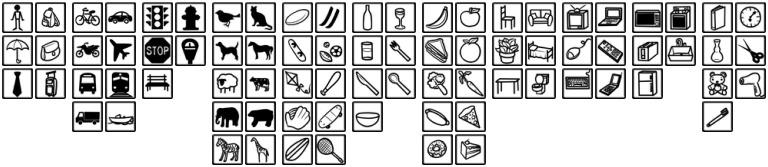
\includegraphics[width=\textwidth]
	{img/coco-classes.png}}
	\caption{\label{fig:input-image} All 80 classes from COCO dataset 2017}
\end{figure}

The COCO dataset not only contains bounding boxes and binary masks for object detection and segmentation, it also includes informations for keypoint estimation, panoptic segmentation and image captioning tasks. It is one of the big baselines for object detection tasks for many years now.

In the end, 42 different images from the four artists Urs Wehrli, Andreas Gursky, David LaChapelle and Jeff Wall has been gathered. Urs Wehrli, the swiss artist behind "Kunst aufräumen" was asked to give his permission to use his images for this project. Thankfully he gave permission to do so. The dataset has then been examined with different object segmentation models on Google Colab.

Google Colab is a free to use infrastructure, powered by Google, that offers a zero-configuration Python and Jupyter environment. Running on Linux Ubuntu with the latest Nvidia GPUs this is a good option to get started with deep learning, as there are also a lot of notebooks about every single kind of neural network tasks available.

\section{Model selection}

With the gathered dataset, different object segmentation models from different frameworks have been tried out on the dataset in inference mode. All these models have been pretrained on the COCO-dataset.
The tried out models were: Mask R-CNN, CenterNet, Detectron2 and ShapeMask. In general, Mask R-CNN outperformed the other models, when inference is run on the dataset. Detectron2 also delivered a good performance but it threw an error when running on many images in a loop on Google Colab.

\section{Framework selection}

At the same time different frameworks have been tested out. These were Tensorflow from Google, Detectron from Facebook and MMDetection, which is a part of the OpenMMLab project developed by Multimedia Laboratory by the Chinese University of Hong Kong. All these frameworks do at least contain one Mask R-CNN model. MMDetection has been chosen as the framework to develop the project in, because it worked out-of-the box when tried out on Google Colab. It returned results when running in inference mode on our dataset in about seven Minutes. MMDetection has a vast number of state-of-the-art models for computer vision tasks available and offers a high-level API that speeds up its usage. It is built on top of PyTorch (primarily developed by Facebook) and delivers a very good performance.

\section{Choosing the programming language}

Because most of the deep-learning frameworks are using Python and also of its ease of use, Python has been used as the sole programming language to develop this project. In addition Python does offer a lot of visual computing libraries that were used to create the tidied up image.

\section{Creating the tidied up image}

After the dataset has been collected, and the model and the framework have been chosen, the next step was to extract all single objects from the output of the model when running in inference mode on an image. Mask R-CNN model outputs for every input image among other things a list with with each a list of bounding boxes, masks, confidence score and predicted class of all objects found in the image. These four results were saved in a list object. The output is per default limited to 100 objects per image. The confidence score was used to filter all objects to get the objects with the highest quality as predicted by the model. The binary mask of the found objects was then applied to the image, creating binary images of the object. An example can be seen here:

\begin{figure}[H]
	\center{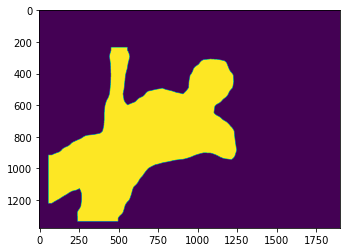
\includegraphics[width=\textwidth]
	{img/binary-mask.png}}
	\caption{\label{fig:binary-mask} Sample binary mask image}
\end{figure}

With help of the binary masks, the background of the found object was coloured white whereas the foreground stayed as is. Subsequently the corresponding bounding boxes were taken to cut out the objects from the image. The last step is to create a grid with all the found objects. This was done with the help of Python's Matplotlib. The idea is to create a grid with the number of rows according to the number of classes and insert every object as a new column. The problem with using Matplotlib's. \texttt{plt.subplots} is that it creates a grid where every image has the same size. To circumvent this, a more complicated approach was taken, by creating a grid manually with the help of the width and the height of all the found objects. A sample input of a tidied up image together with its output can be seen here:

\begin{figure}[H]
    \centering
    \subfloat{{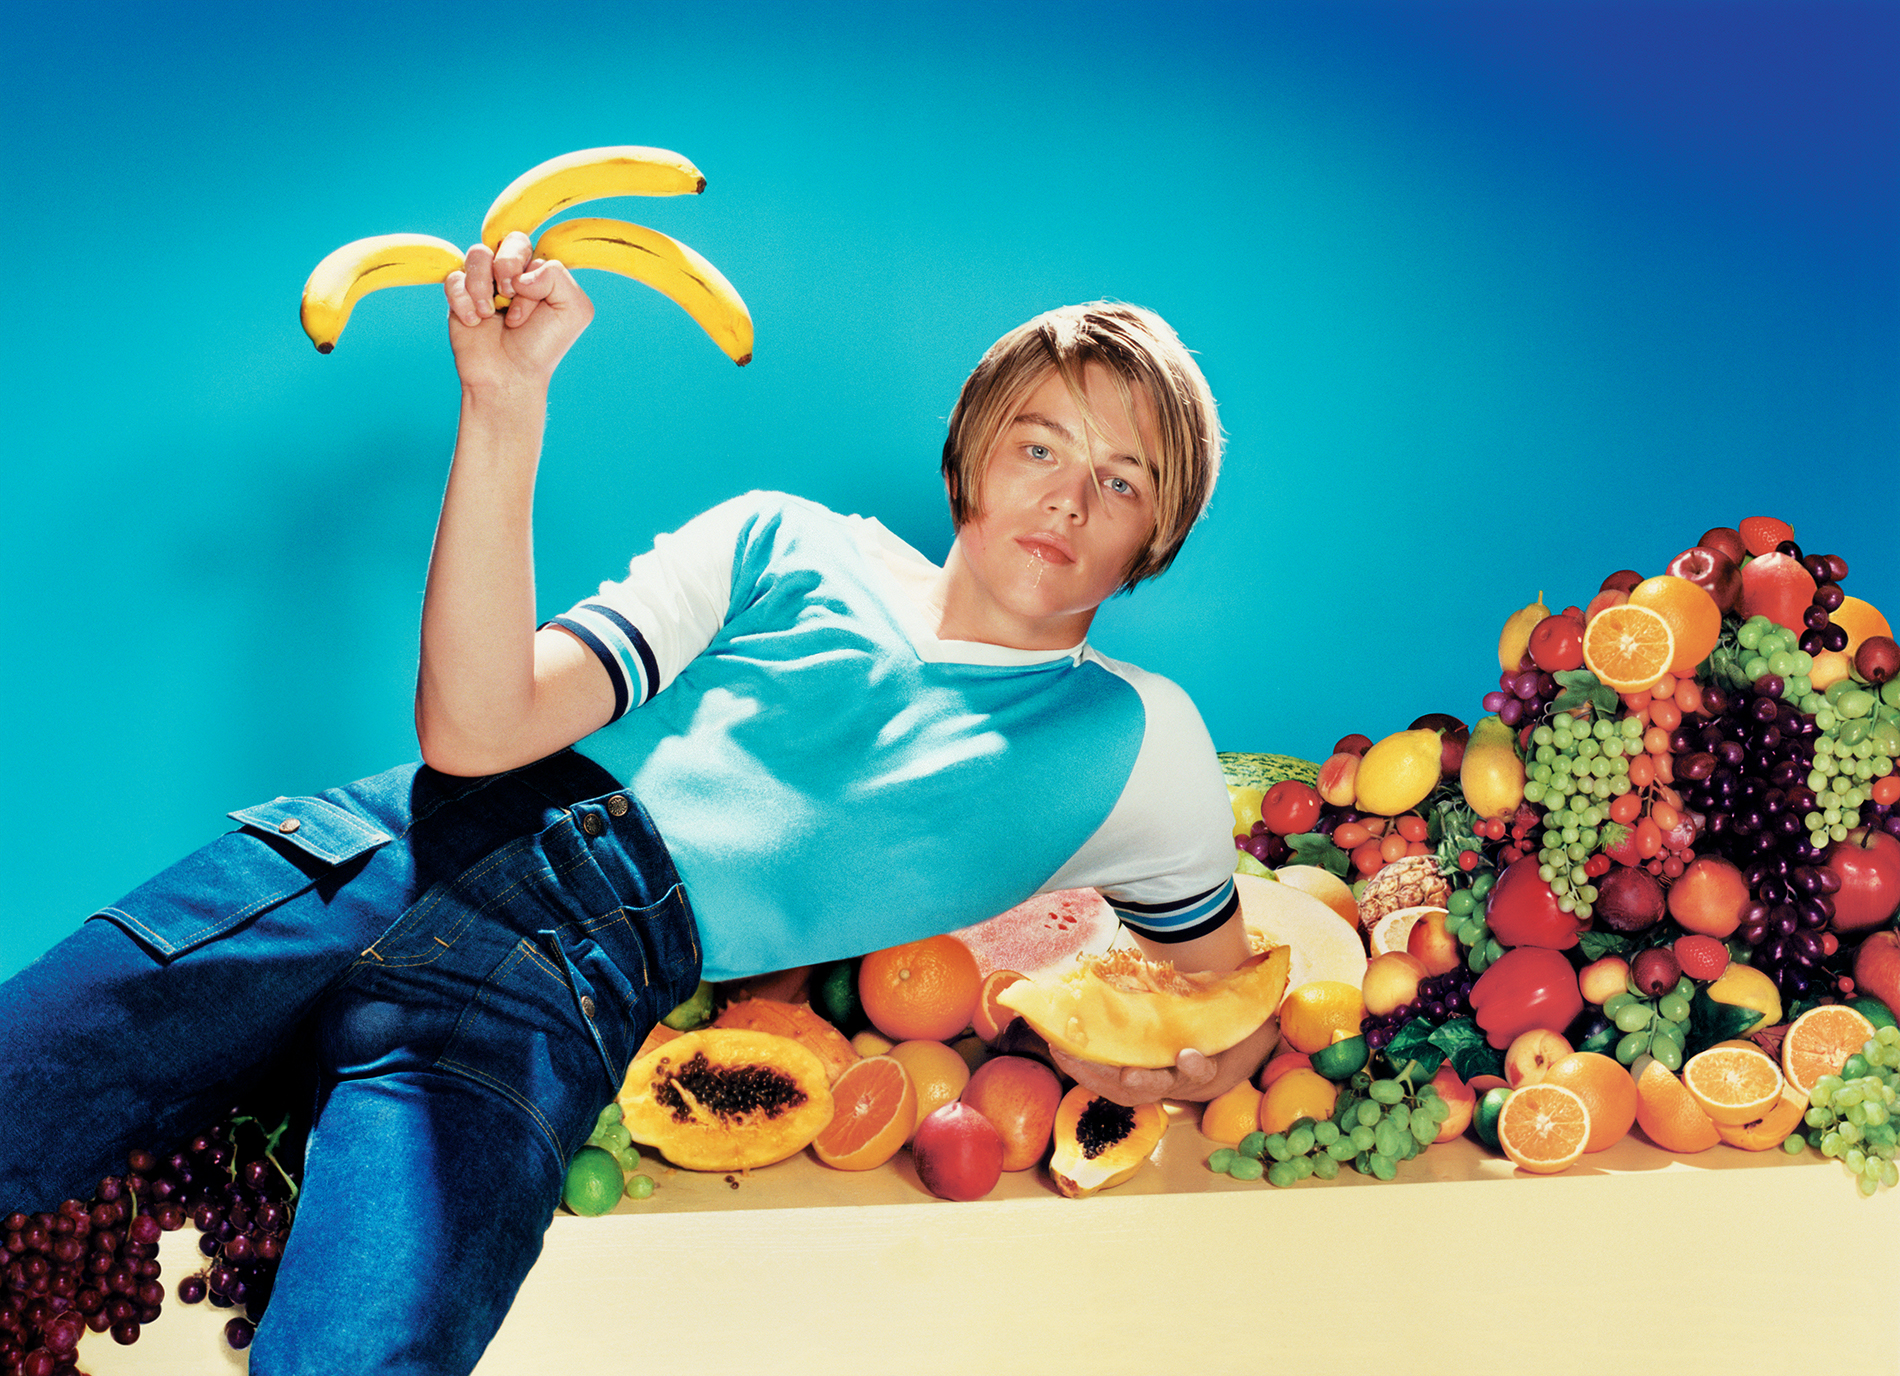
\includegraphics[width=0.5\textwidth]{img/sample-dl-input.jpg} }}
    \subfloat{{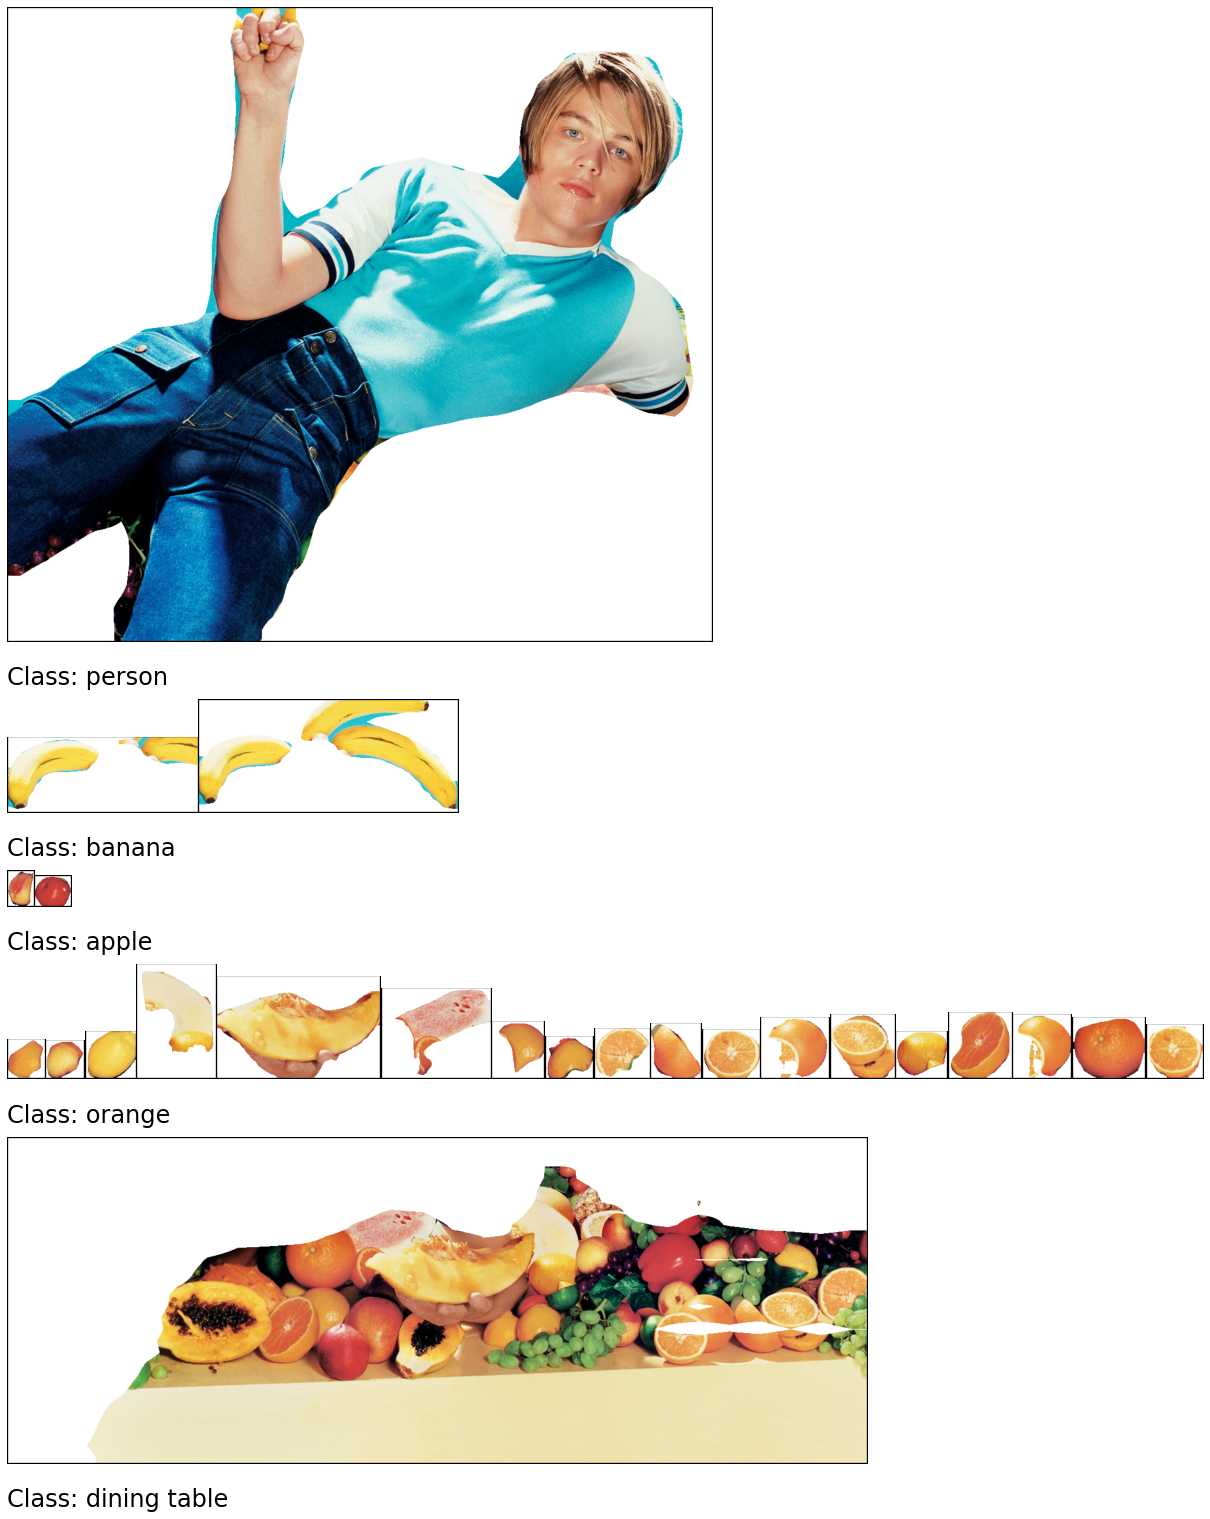
\includegraphics[width=0.5\textwidth]{img/sample-dl-output.png} }}
    \caption{\label{fig:sample-input-output} Sample input and output image}
\end{figure}

\section{Building the application}

After completing the tidied up image, the next step was to build an application that can load an image, run the model in inference mode and return the tidied up image from the input image. A difficulty was that MMDetection, like most deep learning frameworks, needs a Nvidia GPU to run even in inference mode. To solve this problem, a wrapper called SMD was used, that takes in MMDetection models and can run the inference on an arbitrary CPU. \cite{SMD}

To convert the program into a full-blown web application, a framework, called Plotly-Dash has been used. Plotly-Dash is using Flask to create a webserver and is using HTML-, CSS- and JavaScript-technologies under the hood to create a running web application from a Python program. It offers out-of-the-box user interface (UI) components, that are useful to rapid prototype a web application. With the help of UI-elements like buttons and dropdown-lists, the user is given the possibility to upload and select images and models and to start the inference by himself. There are also two sliders built in: One to adjust the confidence threshold score of the model and one to adjust the input image size. Executed time was measured and gets written too to get an insight into performance of the model.

One of the goals of the web application was to build it as modular as possible. This was achieved with the possible selection of the model and three ways to select an image from (predefined list, upload and retrieve via URL). One difficulty with Plotly-Dash was that images when uploaded to the web server, got encoded with base64 encoding. It took some time to find out, how to decode them for further use. A screenshot showing the web application and its UI can be seen here:

 \begin{figure}[H]
	\center{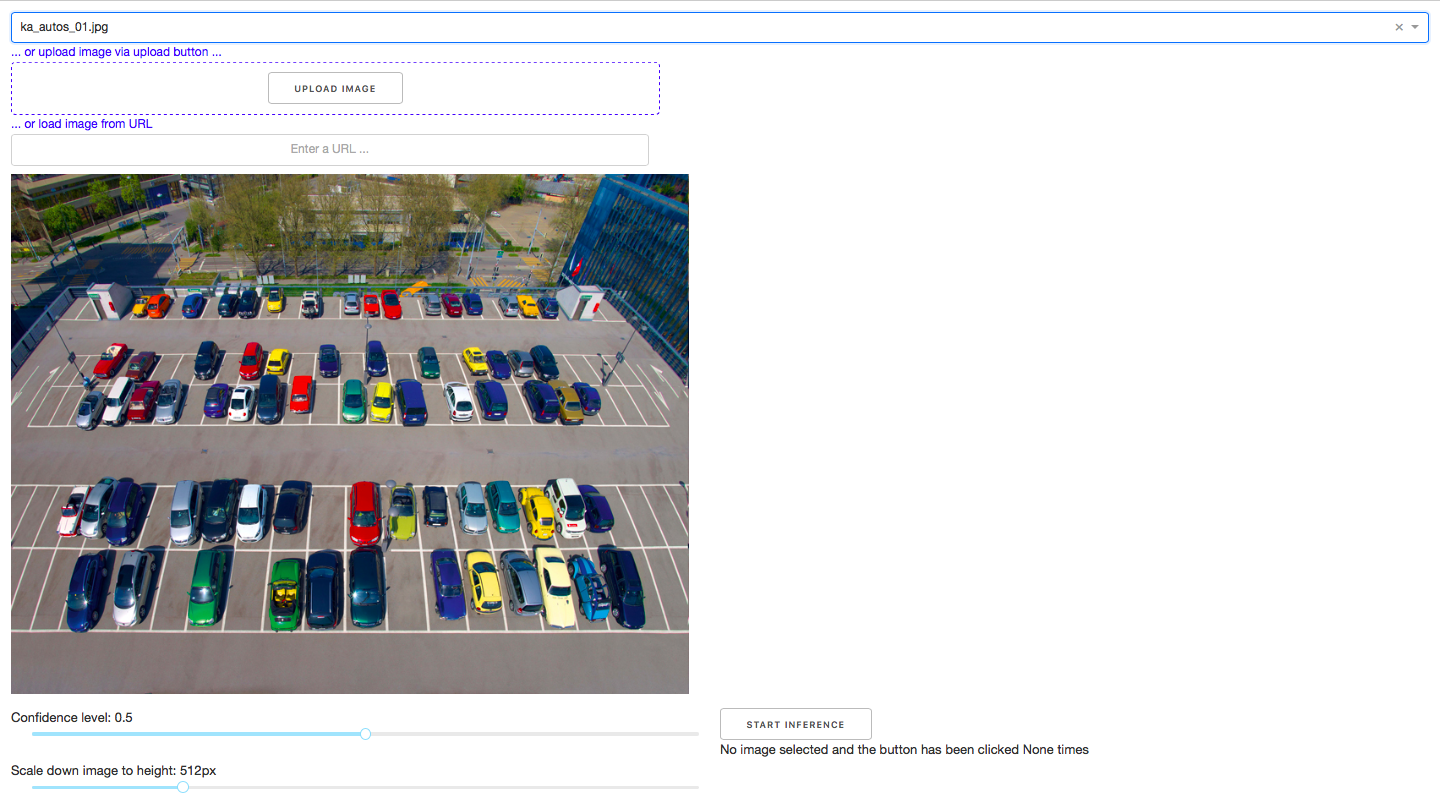
\includegraphics[width=\textwidth]
	{img/web-app-ui.png}}
	\caption{\label{fig:web-app-ui} Screenshot of the webapplication}
\end{figure}

\section{Deployment}

To deploy the application, server space on the EnterpriseLab has been allocated. The web application can be accessed at: \url{http://bdaf20-iameyer.enterpriselab.ch}.

\section{Data labelling}

A dataset containing of three images from the series "Kunst aufräumen" by Urs Wehrli has been chosen to refine the model. As each of these three images contains a messy and a tidy version, it does make a good template to use the tidied up version as a training image and the messy version as a test image. To accomplish training with own images, one has to label these images first. When training an object segmentation model, it is necessary to train the classifier with images that contain masks in it. There are several tools that offer object masking with polygons or brushes. A total of six images (three messy ones and three tidy ones) have been labelled in order to use for refining the model. During labelling, a .xml-file gets generated, that after completion can be converted into the COCO-format as a .json-file.

\section{Refining the model}

Google Colab was used again as the platform to retrain the model. With just three training images it is quite extreme to train a classifier. This reflected in the poor performance in the beginning. After deciding to retrain a single model for every picture pair (messy and tidy one), performance got better. For a task like this, when training with a small dataset, data-augmentation is crucial: It lets the model use the same image over and over again after applying different kind of transformations and distortions to it.

When retraining with MMDetection, one has to adjust several things: A .json-file, containing all the classes, masks and bounding boxes in COCO-format. And a config.py-file that contains all the needed settings for the training process. During retraining, checkpoint-files get saved in a defined interval. These checkpoint-files can be used resume training on a later point of time. After one training cycle (between 1000 and 2000 epochs), the latest checkpoint-file was taken and examined on the test-image.

\section{Results}

Hello